
\begin{figure}
%     \footnotesize
%     \setlength{\unitlength}{\textwidth}
% %     \begin{tikzpicture}(1, 0.6)(0, 0)
% %         \put(0,0){\includegraphics[width=0.99\textwidth]{ccrig/img/fig1_full_v2-crop.pdf}}

% %         % \linethickness{0.1mm}
% %         \put(0.15, 0.44){\vector(1, 0){0.08}}

% %         \put(0.25,0.53){\parbox{1.0in}{1. Collect random interaction samples}}
% %         \put(0.27, 0.38){
\includegraphics[width=0.1\textwidth]{ccrig/img/database_symbol.png}}
% %         \put(0.25, 0.36){$\{ \tau_1, \tau_2, \dots, \tau_N \}$}
% %         \put(0.4, 0.44){\vector(1, 0){0.14}}

% %         \put(0.6,0.55){\parbox{2.0in}{2. Train context-conditioned VAE}}
% %         \put(0.57, 0.34){\includegraphics[width=0.4\textwidth]{ccrig/img/fig1_v6-crop-transparent.png}}

% %         \put(0.03,0.24){\parbox{2.3in}{3. Training phase: agent generates reachable goals
% % and learns policy to minimize latent distance to goal}}
% %         \put(0.54,0.25){\parbox{2.3in}{4. Testing phase: human provides goal image and
% % agent executes policy to reach goal}}
% %     \end{tikzpicture}

%     \begin{picture}(1, 0.6)(0, 0)
%         \put(0,0){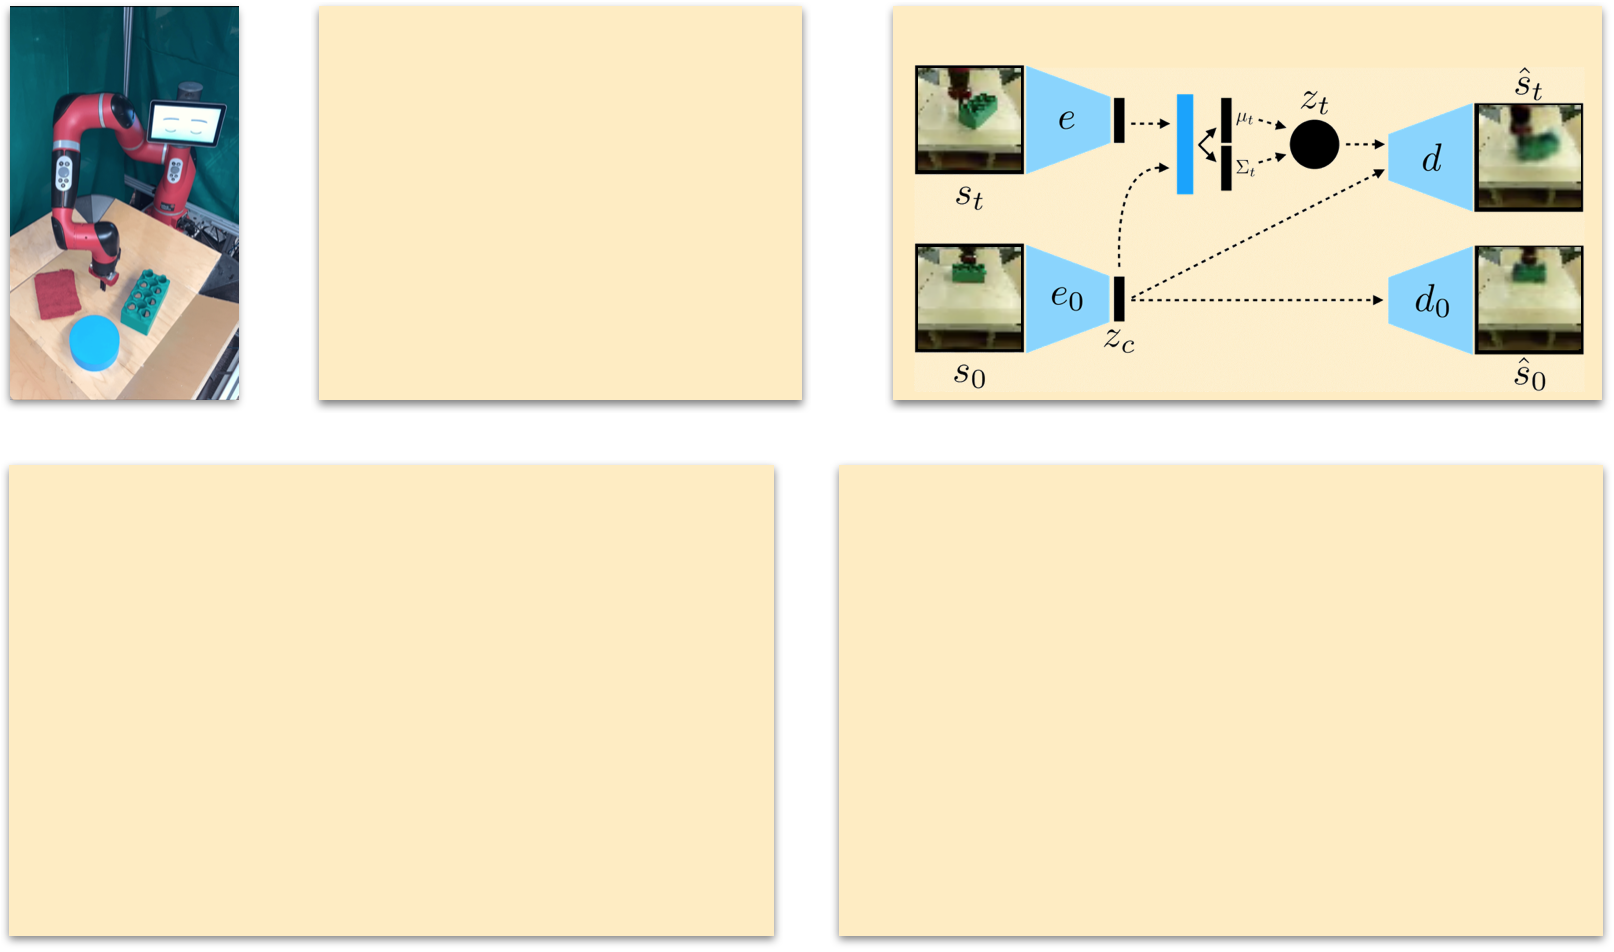
\includegraphics[width=0.99\textwidth]{ccrig/img/fig1_v5b.png}}

%         % \linethickness{0.1mm}
%         \put(0.15, 0.44){\vector(1, 0){0.08}}

%         \put(0.25,0.53){\parbox{1.0in}{1. Collect random interaction samples}}
%         \put(0.27, 0.38){
\includegraphics[width=0.1\textwidth]{ccrig/img/database_symbol.png}}
%         \put(0.25, 0.36){$\{ \tau_1, \tau_2, \dots, \tau_N \}$}
%         \put(0.4, 0.44){\vector(1, 0){0.14}}
%         \qbezier(0.24, 0.365)(0.16, 0.365)(0.16, 0.31)
%         \put(0.16, 0.31){\vector(0, -1){0.01}}

%         \put(0.605,0.555){\parbox{2.0in}{2. Train context-conditioned VAE}}
%         % \put(0.57, 0.34){\includegraphics[width=0.4\textwidth]{ccrig/img/fig1_v6-crop-transparent.png}}
%         \qbezier(0.66, 0.35)(0.66, 0.32)(0.6, 0.32)
%         \put(0.6, 0.32){\line(-1,0){0.40}}
%         \qbezier(0.20, 0.32)(0.18, 0.32)(0.18, 0.31)
%         \put(0.18, 0.31){\vector(0, -1){0.01}}
%         % \put(0.4, 0.31){$e, e_0$}

%         \put(0.03,0.25){\parbox{2.3in}{3. RL training: learn policy $\pi(\bar{z}_t, \bar{z}_g)$ to minimize latent distance to generated goal $z_g$}}
%         \put(0.03,0.11){
%             \parbox{2.3in}{
%                 % \vspace{0.1cm}

%                 \hspace{0.04\linewidth} $s_0$ \hspace{0.575\linewidth} $s_H$ \hspace{0.065\linewidth} $d(\bar{z}_g)$

%                 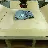
\includegraphics[width=0.15\linewidth]{ccrig/img/real_vae_rollout_new/0/0.png}
%                 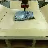
\includegraphics[width=0.15\linewidth]{ccrig/img/real_vae_rollout_new/0/1.png}
%                 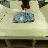
\includegraphics[width=0.15\linewidth]{ccrig/img/real_vae_rollout_new/0/2.png}
%                 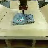
\includegraphics[width=0.15\linewidth]{ccrig/img/real_vae_rollout_new/0/3.png}
%                 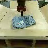
\includegraphics[width=0.15\linewidth]{ccrig/img/real_vae_rollout_new/0/4.png}
%                 \hspace{0.02\linewidth}
%                 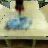
\includegraphics[width=0.15\linewidth]{ccrig/img/real_vae_rollout_new/0/goal.png}

%                 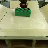
\includegraphics[width=0.15\linewidth]{ccrig/img/real_vae_rollout_new/1/0.png}
%                 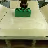
\includegraphics[width=0.15\linewidth]{ccrig/img/real_vae_rollout_new/1/1.png}
%                 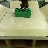
\includegraphics[width=0.15\linewidth]{ccrig/img/real_vae_rollout_new/1/2.png}
%                 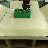
\includegraphics[width=0.15\linewidth]{ccrig/img/real_vae_rollout_new/1/3.png}
%                 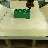
\includegraphics[width=0.15\linewidth]{ccrig/img/real_vae_rollout_new/1/4.png}
%                 \hspace{0.02\linewidth}
%                 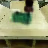
\includegraphics[width=0.15\linewidth]{ccrig/img/real_vae_rollout_new/1/goal.png}

%                 \vspace{0.05cm}

%                 \hspace{0.08\linewidth} Real-world Pusher Training Rollouts
%             }
%         }

%         \put(0.47, 0.14){\vector(1, 0){0.04}}

%         \put(0.54,0.25){\parbox{2.3in}{4. Test time: agent executes policy to reach human-provided goal image $s_g$}}
%         \put(0.54,0.11){
%             \parbox{2.3in}{
%                 % \vspace{0.1cm}

%                 \hspace{0.04\linewidth} $s_0$ \hspace{0.575\linewidth} $s_H$ \hspace{0.1\linewidth} $s_g$

%                 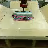
\includegraphics[width=0.15\linewidth]{ccrig/img/real_env_rollout_novel/2/0.png}
%                 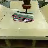
\includegraphics[width=0.15\linewidth]{ccrig/img/real_env_rollout_novel/2/1.png}
%                 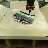
\includegraphics[width=0.15\linewidth]{ccrig/img/real_env_rollout_novel/2/2.png}
%                 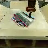
\includegraphics[width=0.15\linewidth]{ccrig/img/real_env_rollout_novel/2/3.png}
%                 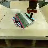
\includegraphics[width=0.15\linewidth]{ccrig/img/real_env_rollout_novel/2/4.png}
%                 \hspace{0.02\linewidth}
%                 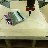
\includegraphics[width=0.15\linewidth]{ccrig/img/real_env_rollout_novel/2/goal.png}

%                 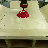
\includegraphics[width=0.15\linewidth]{ccrig/img/real_env_rollout_novel/3/0.png}
%                 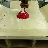
\includegraphics[width=0.15\linewidth]{ccrig/img/real_env_rollout_novel/3/1.png}
%                 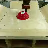
\includegraphics[width=0.15\linewidth]{ccrig/img/real_env_rollout_novel/3/2.png}
%                 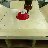
\includegraphics[width=0.15\linewidth]{ccrig/img/real_env_rollout_novel/3/3.png}
%                 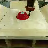
\includegraphics[width=0.15\linewidth]{ccrig/img/real_env_rollout_novel/3/4.png}
%                 \hspace{0.02\linewidth}
%                 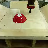
\includegraphics[width=0.15\linewidth]{ccrig/img/real_env_rollout_novel/3/goal.png}

%                 \vspace{0.05cm}

%                 \hspace{0.15\linewidth}
%                 Test Rollouts (Unseen Objects)
%             }
%         }
%     \end{picture}
    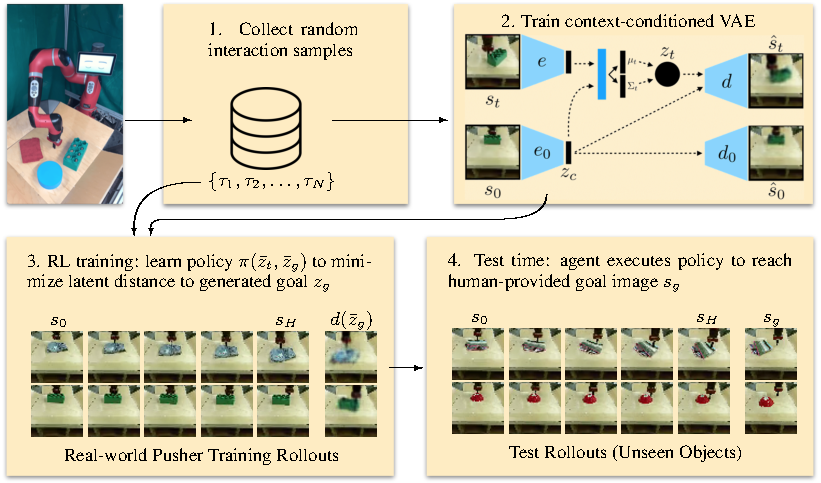
\includegraphics[width=\linewidth]{ccrig/fig1.pdf}

    \caption{System overview of our self-supervised learning algorithm.
    (1) The agent collects random interaction data, to be used for both representation learning and as additional off-policy data for RL.
    (2) We propose a context-conditioned generative model (CC-VAE) to learn generalizable skills.
    In order to improve the generation of plausible goal states that result from a starting state $s_0$, our model allows information to flow freely through the context $z_c$ while an information bottleneck on $z_t$ gives us the ability to generate samples by re-sampling only $z_t$.
    % Meanwhile, information is free to flow through $z_t$.
    This architecture provides a compact representation of the scene disentangling information that changes within a rollout ($z_t$) and information that changes between rollouts ($z_c$).
    We then use $\bar{z}_t = (z_t, z_c)$ as the representation for RL.
    (3) Our proposed CC-RIG algorithm samples latent goals, using the above representation, and learns a policy to minimize the latent distance to the goal with off-policy RL.
    Rollouts are shown on the real-world Sawyer robot pusher environment with visual variation.
    We include the initial image $s_0$, selected frames from the rollout, final image $s_H$, and the decoded goal latent $d(\bar{z}_g)$.
    (4) At test time, the agent is given a goal image $s_g$ and executes the policy to reach it. Our method successfully handles pushing novel objects that were unseen at training time. Example rollouts can be found at  \url{https://ccrig.github.io/}}
    % \vspace{-0.4in}
    \label{fig:fig1}
\end{figure}
